%*----------- SLIDE -------------------------------------------------------------
\begin{frame}[t]{Introdução} 
    \transdissolve[duration=0.5]
    Um dos pontos importantes na área da robótica móvel é a localização e mapeamento de locais desconhecidos, através dos sistemas SLAM é possível construir um mapa do ambiente e, ao mesmo tempo, usar esse mapa para calcular sua localização.
    

    A comparação é feita através dos seguintes sensores:
    %\newline
        \begin{columns}[t]
            \column{.05\linewidth}
            \column{.4\linewidth}
                \begin{enumerate}
                    \item Lidar 2D; 
                    \item Câmera monocular;
                    \item Câmera stéreo.
                \end{enumerate}
            \column{.6\linewidth}
            \begin{center}
            %\centerline{
                \begin{figure}
                    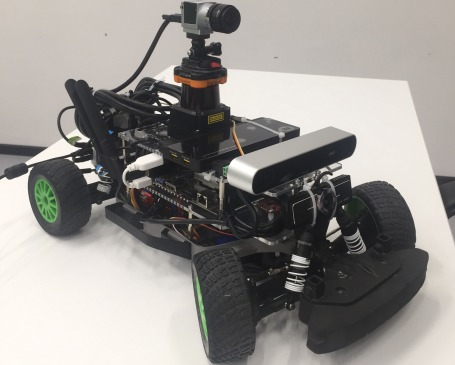
\includegraphics[width=0.45\textwidth]{pista}
                    \caption{ \cite{filipenko2018comparison}}
                \end{figure}
            %}
            \end{center}
        \end{columns}
%*----------- notes
    \note[item]{Notes can help you to remember important information. Turn on the notes option.}
\end{frame}
%-
%*----------- SLIDE -------------------------------------------------------------
\begin{frame}[c]{Objetivo} 
    %\framesubtitle{sub-objetivo}
    \transdissolve[duration=0.5]
   
    \begin{center}
        \Wider{%
        \begin{shaded}
        \begin{center}
            \vspace*{0.5cm}
            \resizebox{!}{0.5cm}{%
                \color{bg} Comparar as trajetórias de cada sistema SLAM
            }%
        \end{center}
        \end{shaded}
        }%
    \end{center}
    
   
%*----------- notes
    \note[item]{Notes can help you to remember important information. Turn on the notes option.}
\end{frame}
%-
%*----------- SLIDE -------------------------------------------------------------
\begin{frame}[t]{Lidar 2D}
    \transboxout[duration=0.5]
    %\framesubtitle{Darwin-OP}
    \begin{columns}
        %\column{.1\textwidth}
        \column{.4\textwidth}
            \begin{figure}
            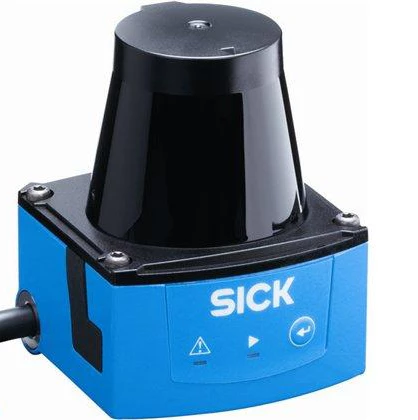
\includegraphics[width=0.9\textwidth]{lidar.png}
            \caption{\cite{Sensores71}}
            \end{figure}
        \column{.4\textwidth}
            \begin{enumerate}
                \item GMAPPING;
                \item Hector SLAM;
                \item Cartographer;     
            \end{enumerate}
    \end{columns}
 %*----------- notes
    %\note[item]{Notes can help you to remember important information. Turn on the notes option.}
\end{frame}
%-
%*----------- SLIDE -------------------------------------------------------------
\begin{frame}[c]{GMAPPING}
    %\transboxin[duration=1,direction=30]
    \transboxout[duration=0.5]
    %\framesubtitle{Darwin-OP}
    \begin{columns}
        %\column{.1\textwidth}
        \column{.6\textwidth}
            \begin{figure}
            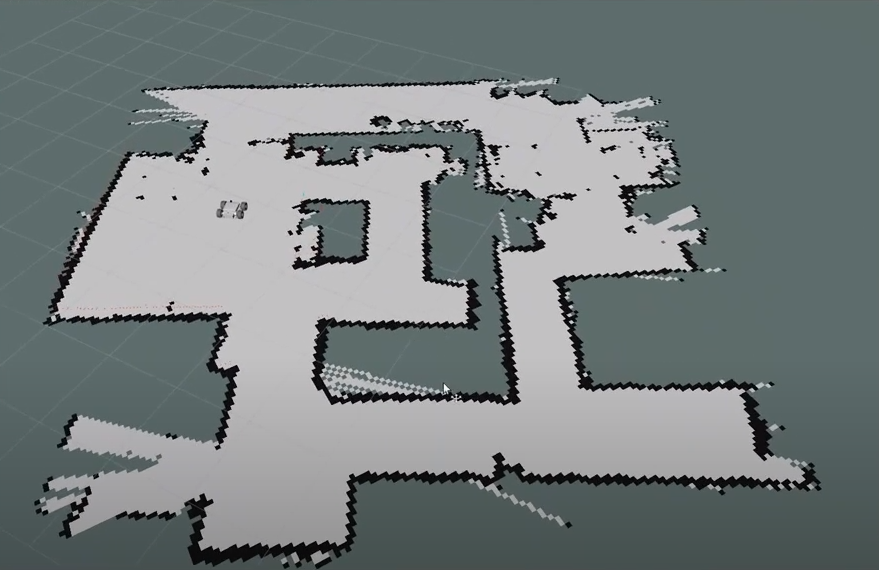
\includegraphics[width=1\textwidth]{gmappp.png}
            \caption{\cite{Robotics19}}
            \end{figure}
        \column{.4\textwidth}
            \begin{enumerate}
                \item É um dos mais usados para aplicações em robôs;
                \item Usa filtro de partículas;
                \item Cria o grid-based map;     
            \end{enumerate}
    \end{columns}

%*----------- notes
    %\note[item]{Notes can help you to remember important information. Turn on the notes option.}
\end{frame}
%-
%*----------- SLIDE -------------------------------------------------------------
\begin{frame}[c]{HECTOR SLAM}
    %\transboxin[duration=1,direction=30]
     %\transboxin[duration=1,direction=30]
    \transboxout[duration=0.5]
    %\framesubtitle{Darwin-OP}
    \begin{columns}
        %\column{.1\textwidth}
        \column{.6\textwidth}
            \begin{figure}
            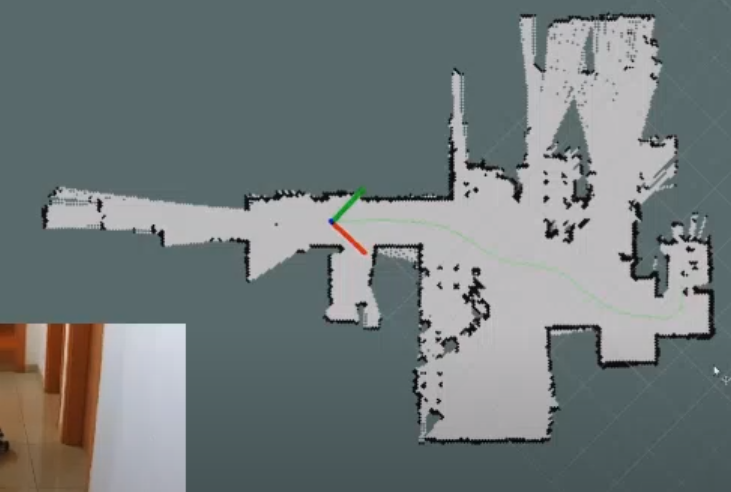
\includegraphics[width=1\textwidth]{hectorrr.png}
            \caption{\cite{HectorSL95}}
            \end{figure}
        \column{.4\textwidth}
            \begin{enumerate}
                \item Produz um mapa bastante preciso;
                \item Combina o método robusto de digitalização e o uso de sistemas de detecção inercial;
                \item Não precisa de hodômetro;  
                \item é possível usa-lo em drones e veículos terrestres operem em locais irregulares. 
            \end{enumerate}
    \end{columns}


%*----------- notes
    %\note[item]{Notes can help you to remember important information. Turn on the notes option.}
\end{frame}
%-
%*----------- SLIDE -------------------------------------------------------------
\begin{frame}[c]{CARTOGRAPHER}
    %\transboxin[duration=1,direction=30]
    \transboxout[duration=0.5]
    %\framesubtitle{Darwin-OP}
    \begin{columns}
        %\column{.1\textwidth}
        \column{.6\textwidth}
            \begin{figure}
            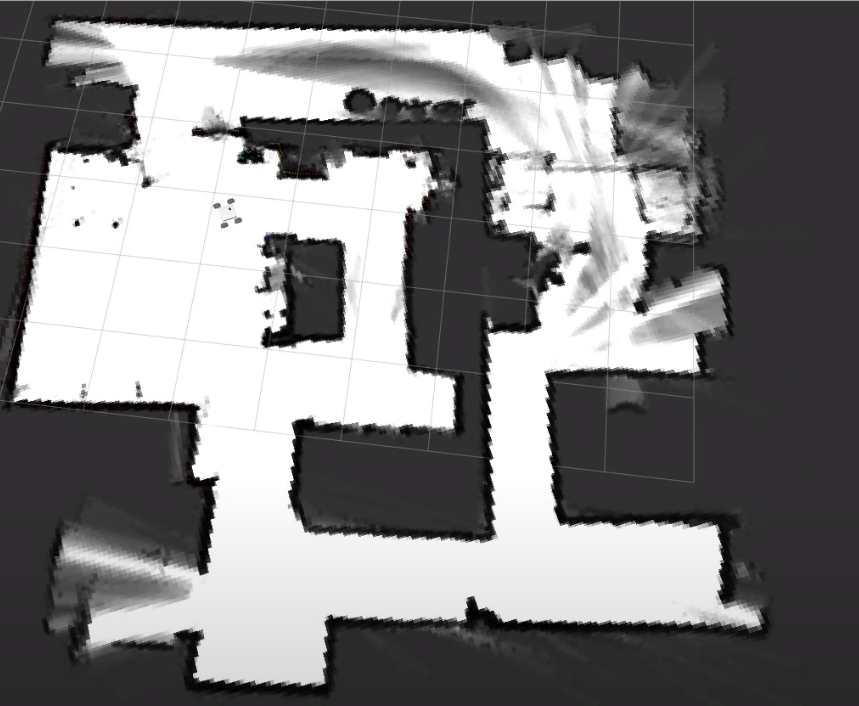
\includegraphics[width=.8\textwidth]{cart.png}
            \caption{\cite{Cartogra48}}
            \end{figure}
        \column{.4\textwidth}
            \begin{enumerate}
                \item Possui um mapeamento interno em tempo real;
                \item Utiliza mapeamento baseado em grade; 
                \item Pode ser usados em varias plataformas como Turtlebot, PR 2, Toyota HSR por causa da integração com o ROS. 
            \end{enumerate}
    \end{columns}

%*----------- notes
    %\note[item]{Notes can help you to remember important information. Turn on the notes option.}
\end{frame}
%-
%*----------- SLIDE -------------------------------------------------------------
\begin{frame}[t]{Comparação}
    \transboxout[duration=0.5]
    %\framesubtitle{Darwin-OP}
    \begin{columns}
        \column{.2\textwidth}
            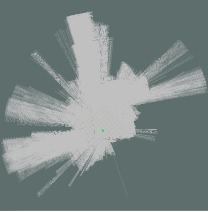
\includegraphics[width=1.2\textwidth]{gmapp.jpeg}
        \column{.2\textwidth}
            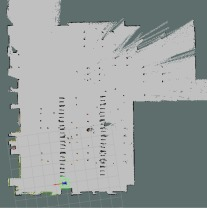
\includegraphics[width=1.2\textwidth]{hectorr.jpeg}
        \column{.2\textwidth}
            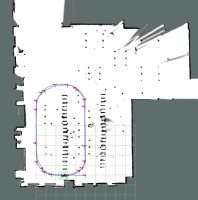
\includegraphics[width=1.2\textwidth]{cartog.jpeg}
        \column{.2\textwidth}
            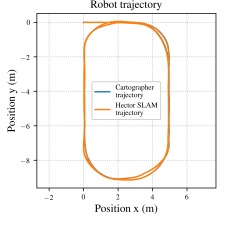
\includegraphics[width=1.2\textwidth]{hxc.jpeg}
    \end{columns}
 %*----------- notes
    %\note[item]{Notes can help you to remember important information. Turn on the notes option.}
\end{frame}
%
%*----------- SLIDE -------------------------------------------------------------
\begin{frame}[t]{Comparação De Resultados}
    %\transboxin[duration=1,direction=30]
    \transboxout[duration=0.5]
    %\framesubtitle{Darwin-OP}
    \begin{columns}
        %\column{.1\textwidth}
        \column{.9\textwidth}
            \begin{enumerate}
                \item GMMAPING - Não apresentou um mapa real do ambiente, a trajetória não pode ser computada pois não existe um mapa robusto do ambiente. Por conta disso não apresentou resultados confiáveis.;
                \item HECTOR SLAM - Produz medições precisas e inclusive pode ser usado para validar a trajetória de outros sistemas SLAM. Utiliza mapeamento baseado em grade; 
                \item CARTOGRAPHER - Mostra melhor ajuste dos mapas 2D , demonstra um bom resultado. 
            \end{enumerate}
    \end{columns}
 %*----------- notes
    %\note[item]{Notes can help you to remember important information. Turn on the notes option.}
\end{frame}
%-
%*----------- SLIDE -------------------------------------------------------------
\begin{frame}[t]{Lidar}
    \transboxout[duration=0.5]
    %\framesubtitle{Darwin-OP}
    \begin{columns}
        \column{1\textwidth}
            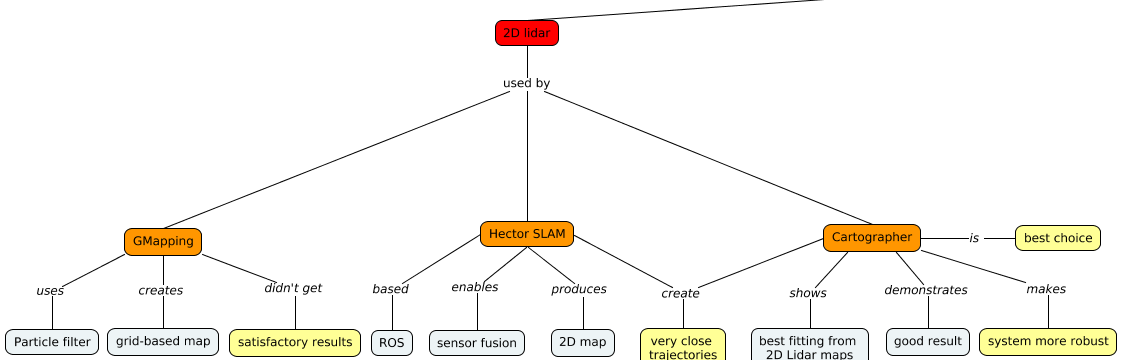
\includegraphics[width=1\textwidth]{lidarr.png}
    \end{columns}
 %*----------- notes
    %\note[item]{Notes can help you to remember important information. Turn on the notes option.}
\end{frame}
%-
%*----------- SLIDE -------------------------------------------------------------
\begin{frame}[t]{Monocular}
    \transboxout[duration=0.5]
    %\framesubtitle{Darwin-OP}
    \begin{columns}
        %\column{.1\textwidth}
        \column{.5\textwidth}
            \begin{figure}
                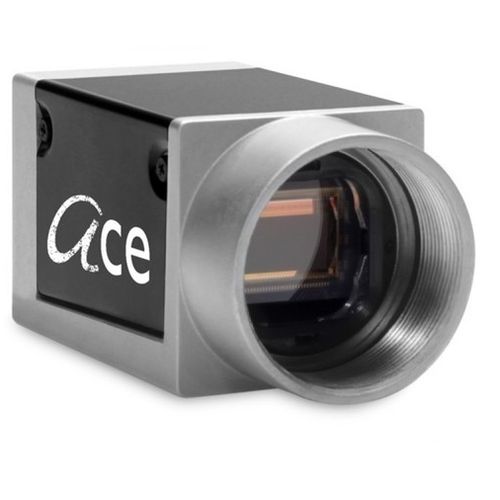
\includegraphics[width=0.7\textwidth]{cameramono.png}
                \caption{\cite{Baslerca30}}
            \end{figure}
        \column{.5\textwidth}
            \begin{enumerate}
                \item Parallel Tracking and Mapping (PTAM);
                \item Semi-direct Visual Odometry (SVO);
                \item Dense Piecewise Parallel Tracking and Mapping (DPP-
                        TAM);
                \item Large Scale Direct monocular SLAM (LSD SLAM);
                \item ORB SLAM (mono);
                \item Direct Sparse Odometry (DSO).
            \end{enumerate}
    \end{columns}
 %*----------- notes
    %\note[item]{Notes can help you to remember important information. Turn on the notes option.}
\end{frame}
%-
%*----------- SLIDE -------------------------------------------------------------
\begin{frame}[c]{Parallel Tracking and Mapping (PTAM):}
    %\transboxin[duration=1,direction=30]
    \transboxout[duration=0.5]
    %\framesubtitle{Darwin-OP}
    \begin{columns}
        %\column{.1\textwidth}
        \column{.6\textwidth}
            \begin{figure}
            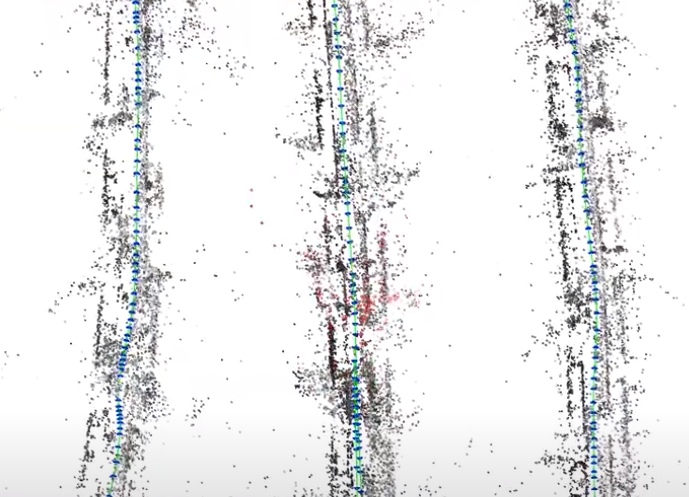
\includegraphics[width=0.9\textwidth]{p.png}
            \caption{\cite{webcite}}
            \end{figure}
        \column{.4\textwidth}
            \begin{enumerate}
                \item Baseado em quadro-chave;
                \item Permite estimar a pose do robô; 
                \item Construir o mapa rastreando características; 
                \item Não produz um para para o ambiente do ROS.
            \end{enumerate}
    \end{columns}
%*----------- notes
    %\note[item]{Notes can help you to remember important information. Turn on the notes option.}
\end{frame}
%-
%*----------- SLIDE -------------------------------------------------------------
\begin{frame}[c]{Semi-direct Visual Odometry (SVO):}
   %\transboxin[duration=1,direction=30]
    \transboxout[duration=0.5]
    %\framesubtitle{Darwin-OP}
    \begin{columns}
        %\column{.1\textwidth}
        \column{.6\textwidth}
            \begin{figure}
            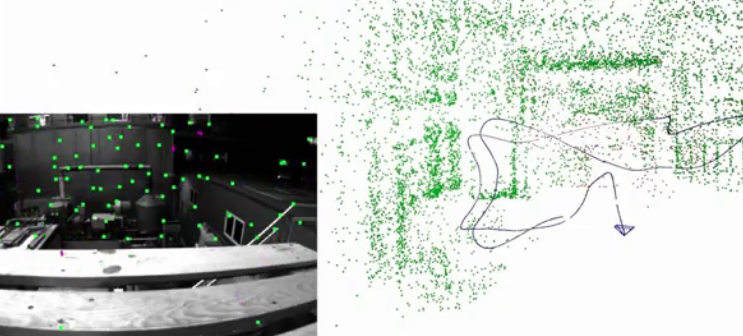
\includegraphics[width=1\textwidth]{svo.png}
            \caption{\cite{SVOFastS44}}
            \end{figure}
        \column{.4\textwidth}
            \begin{enumerate}
                \item Usa um paradigma semi-direto;
                \item Estimar o movimento a partir da intensidade dos pixels; 
                \item Não houve um resultado satisfatório. 
            \end{enumerate}
    \end{columns}
%*----------- notes
    %\note[item]{Notes can help you to remember important information. Turn on the notes option.}
\end{frame}
%-
%*----------- SLIDE -------------------------------------------------------------
\begin{frame}[c]{Dense Piecewise Parallel Tracking and Mapping(DPP-
TAM)}
    %\transboxin[duration=1,direction=30]
    \transboxout[duration=0.5]
    %\framesubtitle{Darwin-OP}
    \begin{columns}
        %\column{.1\textwidth}
        \column{.6\textwidth}
            \begin{figure}
            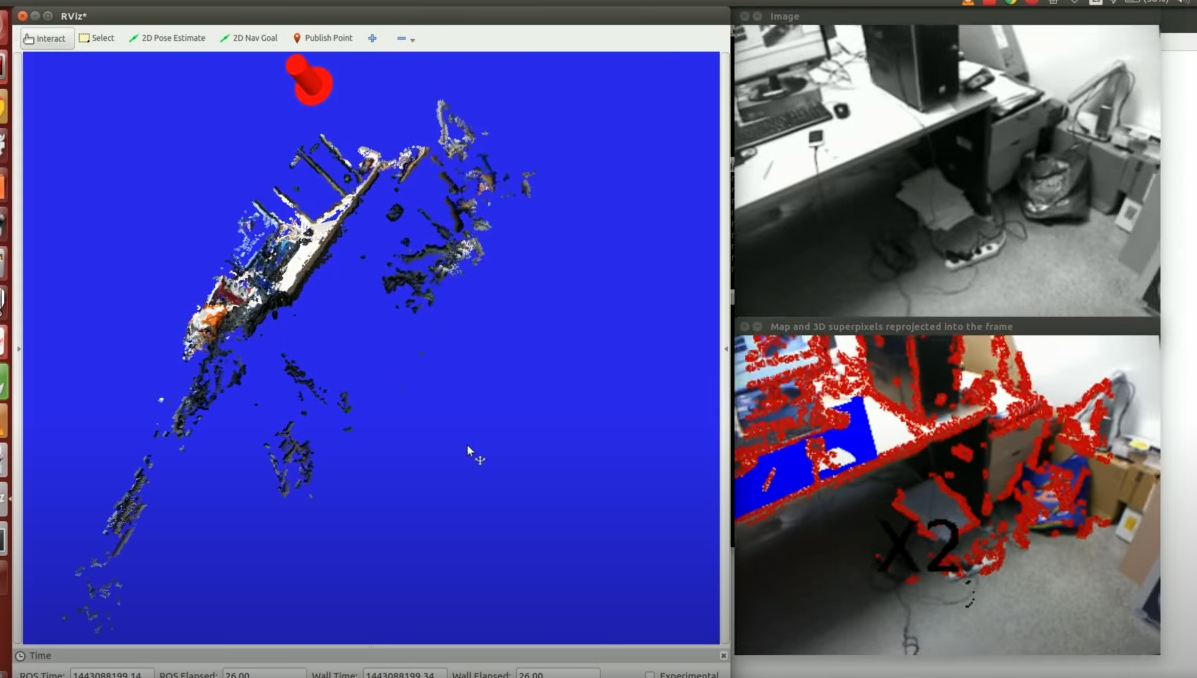
\includegraphics[width=1\textwidth]{DPP.png}
            \caption{\cite{PDFDPPTA82}}
            \end{figure}
        \column{.4\textwidth}
            \begin{enumerate}
                \item utiliza uma hipótese de que as regioes com a mesma cor pertencem a proximidade do mesmo planoUsa um paradigma semi-direto;
            \end{enumerate}
    \end{columns}

%*----------- notes
    %\note[item]{Notes can help you to remember important information. Turn on the notes option.}
\end{frame}
%-
%*----------- SLIDE -------------------------------------------------------------
\begin{frame}[t]{Comparação}
    \transboxout[duration=0.5]
    %\framesubtitle{Darwin-OP}
    \begin{columns}
        \column{.3\textwidth}
            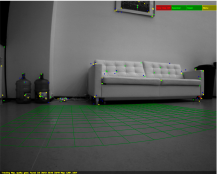
\includegraphics[width=1\textwidth]{PTAM1.png}
        \column{.3\textwidth}
            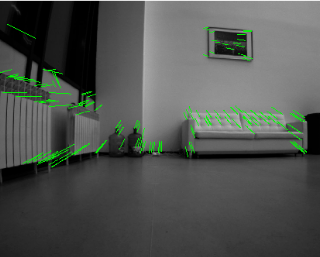
\includegraphics[width=1\textwidth]{SVO1.png}
        \column{.3\textwidth}
            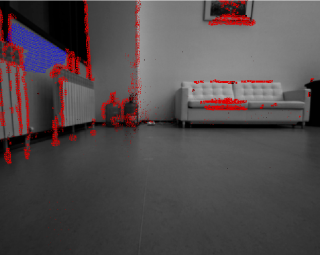
\includegraphics[width=1\textwidth]{DPPTAM1.png}
        
    \end{columns}
 %*----------- notes
    %\note[item]{Notes can help you to remember important information. Turn on the notes option.}
\end{frame}
%-
%*----------- SLIDE -------------------------------------------------------------
\begin{frame}[t]{Comparação De Resultados}
    %\transboxin[duration=1,direction=30]
    \transboxout[duration=0.5]
    %\framesubtitle{Darwin-OP}
    \begin{columns}
        %\column{.1\textwidth}
        \column{.9\textwidth}
            \begin{enumerate}
                \item PTAM - Os resultados não foram confiaveis, o sistema perdeu a pista quando o robô teve uma virada, dessa forma nao é muito robusto nas manobras laterais;
                \item SVO - O sistema não é robusto para esta aplicação ja que o robo perde a pista nas curvas, mas pode ser usado para obter informações dos segmentos de movimentos; 
                \item DPP-TAM - o sistema não é suficientemente robusto para rastreamento em curvas robotizadas. 
            \end{enumerate}
    \end{columns}
 %*----------- notes
    %\note[item]{Notes can help you to remember important information. Turn on the notes option.}
\end{frame}
%-
%*----------- SLIDE -------------------------------------------------------------
\begin{frame}[c]{Large Scale Direct monocular SLAM (LSD SLAM)}
   %\transboxin[duration=1,direction=30]
    \transboxout[duration=0.5]
    %\framesubtitle{Darwin-OP}
    \begin{columns}
        %\column{.1\textwidth}
        \column{.6\textwidth}
            \begin{figure}
            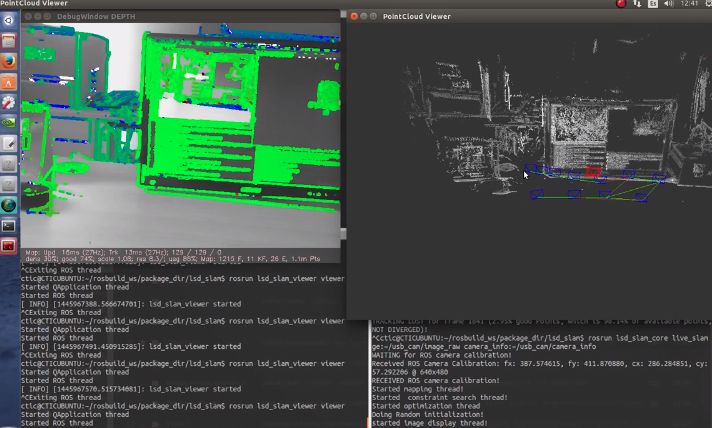
\includegraphics[width=0.9\textwidth]{lsd.png}
            \caption{\cite{LargeSca63}}
            \end{figure}
        \column{.4\textwidth}
            \begin{enumerate}
                \item Utiliza uma imagem local fornecendo uma previsão de pose;
                \item Constrói mapas densos;
                \item Tem fechamento de loop;
                \item Vantagem nos erros de compensação de deriva.
            \end{enumerate}
    \end{columns}

%*----------- notes
    %\note[item]{Notes can help you to remember important information. Turn on the notes option.}
\end{frame}
%-
%*----------- SLIDE -------------------------------------------------------------
\begin{frame}[c]{Direct Sparse Odometry}
    %\transboxin[duration=1,direction=30]
    \transboxout[duration=0.5]
    %\framesubtitle{Darwin-OP}
    \begin{columns}
        %\column{.1\textwidth}
        \column{.6\textwidth}
            \begin{figure}
            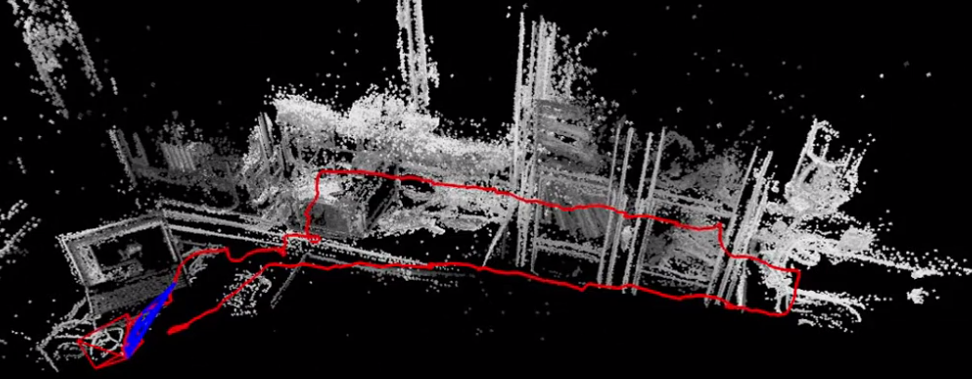
\includegraphics[width=1\textwidth]{dso.png}
            \caption{\cite{DSODirec99}}
            \end{figure}
        \column{.4\textwidth}
            \begin{enumerate}
                \item Precisa de um desenvolvimento adicional para implementação da robótica;
                \item Mapa denso;
                \item sem o fechamento de loop a pose foi acumulada na 1 volta e na 2 ele duplicou os objetos podendo levar a erros adicionais.
            \end{enumerate}
    \end{columns}

%*----------- notes
    %\note[item]{Notes can help you to remember important information. Turn on the notes option.}
\end{frame}
%-
%*----------- SLIDE -------------------------------------------------------------
\begin{frame}[c]{ORB SLAM}
    %\transboxin[duration=1,direction=30]
    \transboxout[duration=0.5]
    %\framesubtitle{Darwin-OP}
    \begin{columns}
        %\column{.1\textwidth}
        \column{.6\textwidth}
            \begin{figure}
            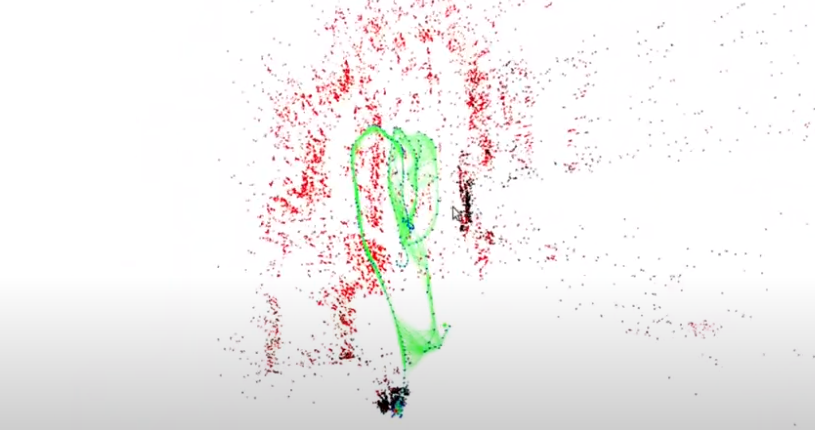
\includegraphics[width=1\textwidth]{orb.png}
            \caption{\cite{ORBSLAM323}}
            \end{figure}
        \column{.4\textwidth}
            \begin{enumerate}
                \item Rastreia as características ORB para estimar a pose do robô;
                \item Cria uma nuvem de pontos como o mapa;
                \item Possui o fechamento de loop para detecção;
                \item Precisa de um desenvolvimento adicional para ser utilizado no ROS.
            \end{enumerate}
    \end{columns}

%*----------- notes
    %\note[item]{Notes can help you to remember important information. Turn on the notes option.}
\end{frame}
%-
%*----------- SLIDE -------------------------------------------------------------
\begin{frame}[t]{Comparação}
    \transboxout[duration=0.5]
    %\framesubtitle{Darwin-OP}
    \begin{columns}
        \column{1\textwidth}
            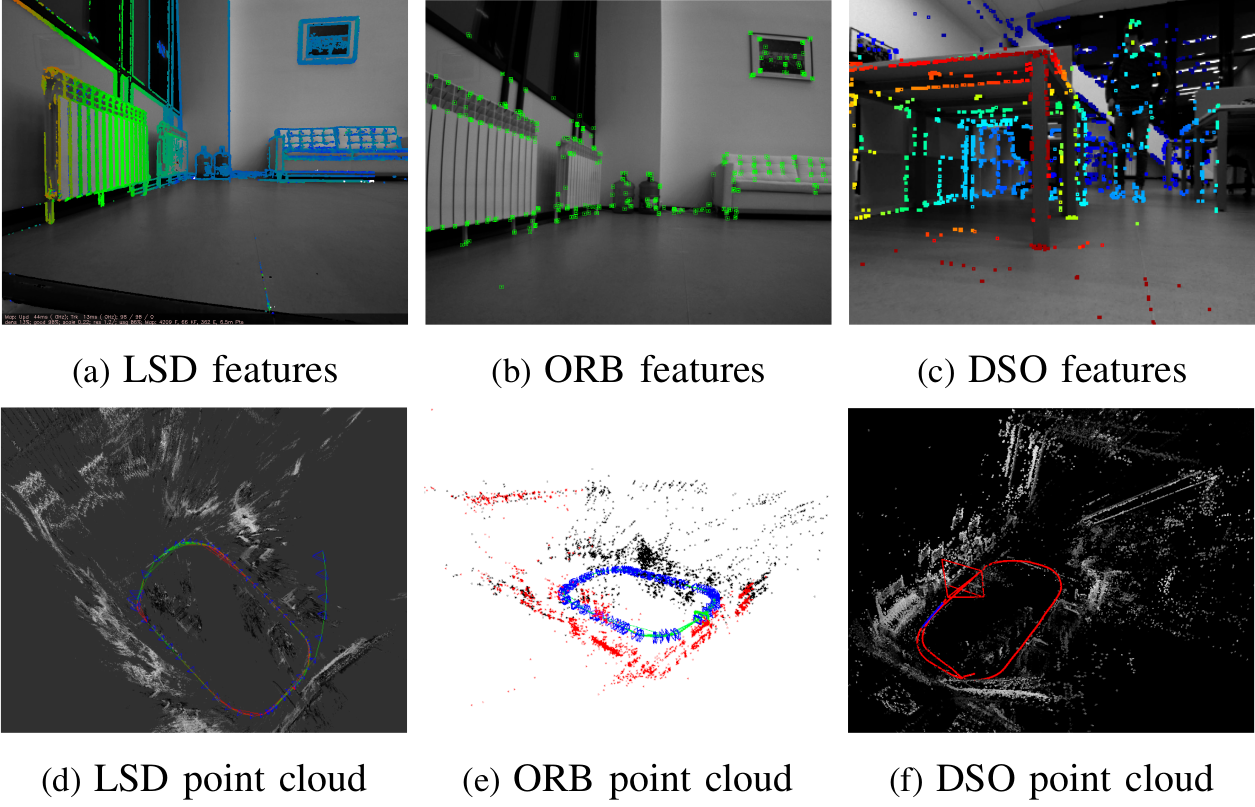
\includegraphics[width=.7\textwidth]{comp.png}       
    \end{columns}
 %*----------- notes
    %\note[item]{Notes can help you to remember important information. Turn on the notes option.}
\end{frame}
%-
%*----------- SLIDE -------------------------------------------------------------
\begin{frame}[t]{Comparação}
    \transboxout[duration=0.5]
    %\framesubtitle{Darwin-OP}
    \begin{columns}
        \column{1\textwidth}
            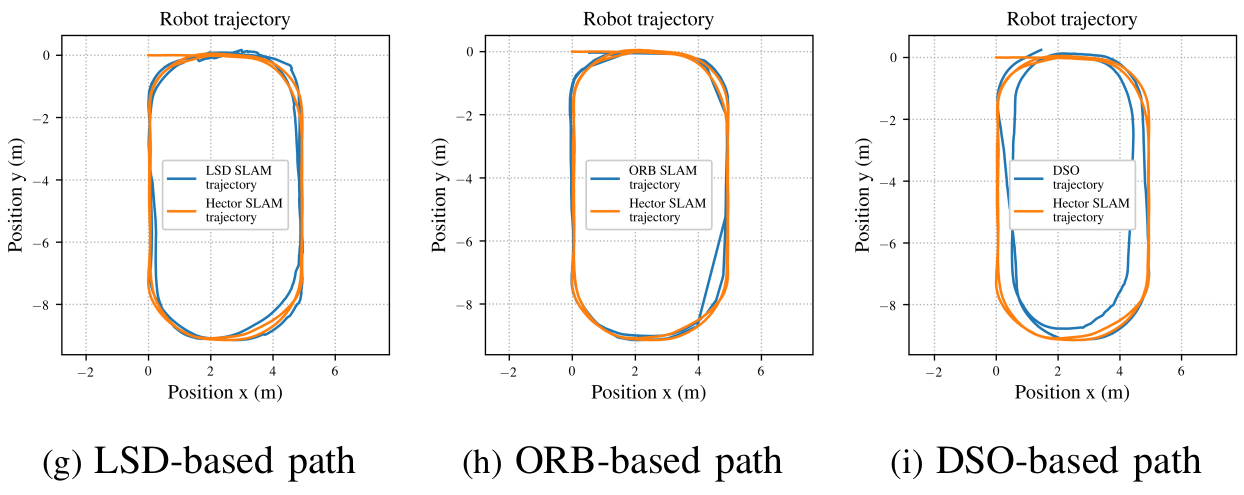
\includegraphics[width=1\textwidth]{compp.png}       
    \end{columns}
 %*----------- notes
    %\note[item]{Notes can help you to remember important information. Turn on the notes option.}
\end{frame}
%-
%*----------- SLIDE -------------------------------------------------------------
\begin{frame}[t]{Comparação De Resultados}
    %\transboxin[duration=1,direction=30]
    \transboxout[duration=0.5]
    %\framesubtitle{Darwin-OP}
    \begin{columns}
        %\column{.1\textwidth}
        \column{.9\textwidth}
            \begin{enumerate}
                \item LSD - Mapa não é suficientemente denso para localização , isso pode ser filtrado com um modelo de movimento robotizado. após a recuperação em escala absoluta pode ser usado para a pose estimada e construção de mapas.
                \item DSO - Cria um mapa denso e é robusto para rastreio de pose mas a falta do fechamento de loop torna o mapa ruidoso, quando adicionado torna o mapa mais preciso.
                \item ORB - Mapa é uma boa aproximação do ambiente, a informação da localização da camera é mais esparsa, é muito robusto  e proporciona uma boa aproximação da trajetória. 
            \end{enumerate}
    \end{columns}
%*----------- notes
    %\note[item]{Notes can help you to remember important information. Turn on the notes option.}
\end{frame}
%-
%*----------- SLIDE -------------------------------------------------------------
\begin{frame}[t]{Camera monocular}
    \transboxout[duration=0.5]
    %\framesubtitle{Darwin-OP}
    \begin{columns}
        \column{1\textwidth}
            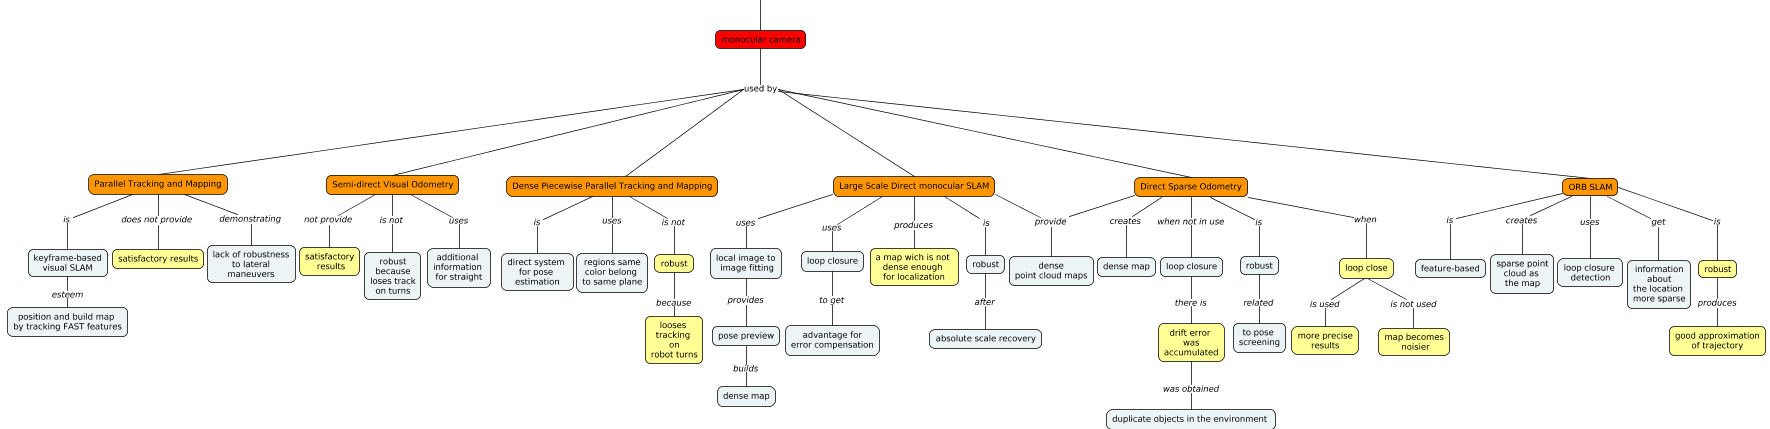
\includegraphics[width=1\textwidth]{monocan.png}
    \end{columns}
 %*----------- notes
    %\note[item]{Notes can help you to remember important information. Turn on the notes option.}
\end{frame}
%-
%*----------- SLIDE -------------------------------------------------------------
\begin{frame}[t]{Camera monocular}
    \transboxout[duration=0.5]
    %\framesubtitle{Darwin-OP}
    \begin{columns}
        \column{1\textwidth}
            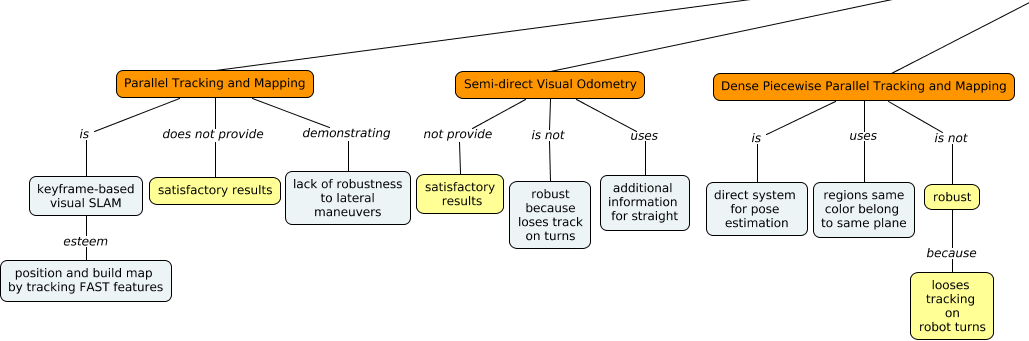
\includegraphics[width=1\textwidth]{monoo.png}
    \end{columns}
 %*----------- notes
    %\note[item]{Notes can help you to remember important information. Turn on the notes option.}
\end{frame}
%-
%*----------- SLIDE -------------------------------------------------------------
\begin{frame}[t]{Camera monocular}
    \transboxout[duration=0.5]
    %\framesubtitle{Darwin-OP}
    \begin{columns}
        \column{1\textwidth}
            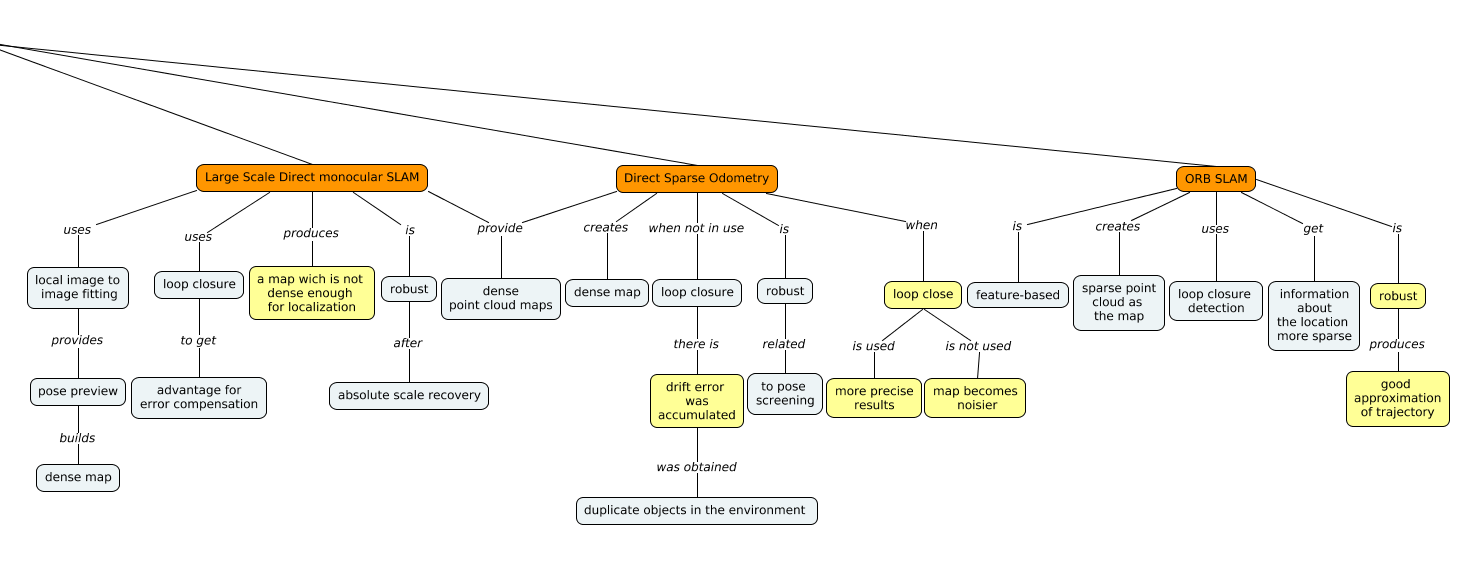
\includegraphics[width=1\textwidth]{comppp.png}
    \end{columns}
 %*----------- notes
    %\note[item]{Notes can help you to remember important information. Turn on the notes option.}
\end{frame}
%-
%*----------- SLIDE -------------------------------------------------------------
\begin{frame}[t]{Câmera stéreo}
    \transboxout[duration=0.5]
    %\framesubtitle{Darwin-OP}
    \begin{columns}
        %\column{.1\textwidth}
        \column{.5\textwidth}
            \begin{figure}
                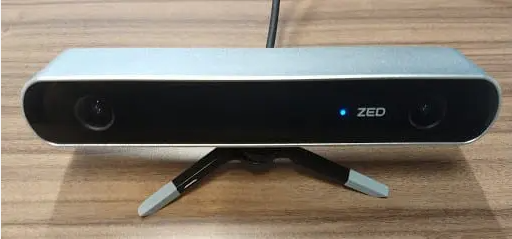
\includegraphics[width=1\textwidth]{stereo.png}
                \caption{\cite{VisualOd23}}
            \end{figure}
        \column{.5\textwidth}
            \begin{enumerate}
                \item ZEDfu;
                \item Real-Time Appearance-Based Mapping;
                \item ORB SLAM;
                \item Stereo Parallel Tracking and Mapping.
            \end{enumerate}
    \end{columns}
 %*----------- notes
    %\note[item]{Notes can help you to remember important information. Turn on the notes option.}
\end{frame}
%-
%*----------- SLIDE -------------------------------------------------------------
\begin{frame}[c]{ZEDfu}
    %\transboxin[duration=1,direction=30]
    \transboxout[duration=0.5]
    %\framesubtitle{Darwin-OP}
    \begin{columns}
        %\column{.1\textwidth}
        \column{.6\textwidth}
            \begin{figure}
            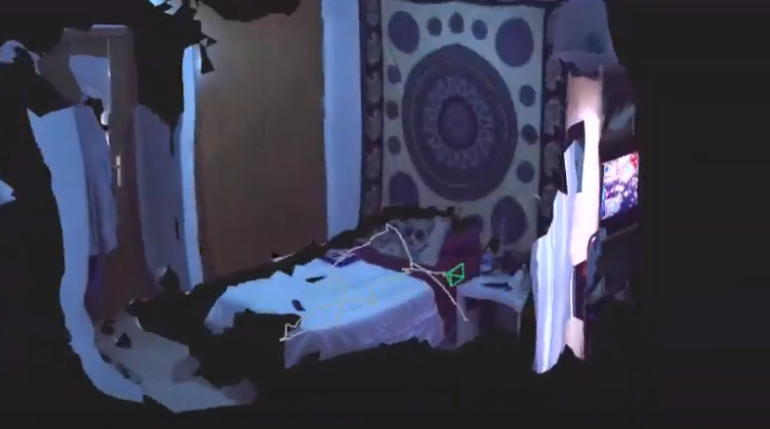
\includegraphics[width=1\textwidth]{zedfu.png}
            \caption{\cite{ZEDfuRea64}}
            \end{figure}
        \column{.4\textwidth}
            \begin{enumerate}
                \item A trajetória é calculada a bordo usando GPU;
            \end{enumerate}
    \end{columns}

%*----------- notes
    %\note[item]{Notes can help you to remember important information. Turn on the notes option.}
\end{frame}
%-

%*----------- SLIDE -------------------------------------------------------------
\begin{frame}[c]{ORB SLAM}
    %\transboxin[duration=1,direction=30]
    \transboxout[duration=0.5]
    %\framesubtitle{Darwin-OP}
    \begin{columns}
        %\column{.1\textwidth}
        \column{.6\textwidth}
            \begin{figure}
            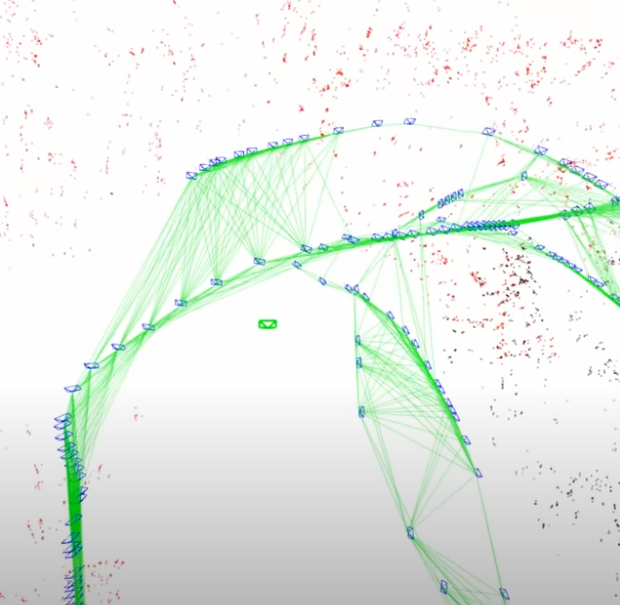
\includegraphics[width=0.6\textwidth]{ORB2.png}
            \caption{\cite{ORBSLAM259}}
            \end{figure}
        \column{.4\textwidth}
            \begin{enumerate}
                \item Pode ser mono ou stéreo;
                \item Fornece escalas absolutas.
            \end{enumerate}
    \end{columns}

%*----------- notes
    %\note[item]{Notes can help you to remember important information. Turn on the notes option.}
\end{frame}
%-
%*----------- SLIDE -------------------------------------------------------------
\begin{frame}[c]{Stereo Parallel Tracking and Mapping}
    %\transboxin[duration=1,direction=30]
    \transboxout[duration=0.5]
    %\framesubtitle{Darwin-OP}
    \begin{columns}
        %\column{.1\textwidth}
        \column{.5\textwidth}
            \begin{figure}
            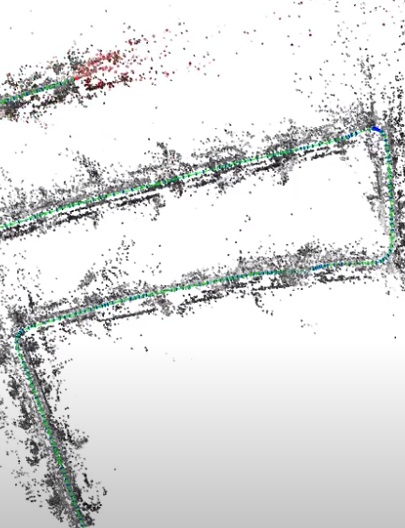
\includegraphics[width=0.6\textwidth]{spt.png}
            \caption{\cite{SPTAMSte99}}
            \end{figure}
        \column{.5\textwidth}
            \begin{enumerate}
                \item Baseado em características;
                \item Tem uma estrutura com detecção de fechamento de loop;
                \item Pode escolher qualquer detector de pontos-chaves disponível no openCV;
                \item Foi testado com e sem fechamento de laço.
            \end{enumerate}
    \end{columns}

%*----------- notes
    %\note[item]{Notes can help you to remember important information. Turn on the notes option.}
\end{frame}
%-
%*----------- SLIDE -------------------------------------------------------------
\begin{frame}[t]{Comparação}
    \transboxout[duration=0.5]
    %\framesubtitle{Darwin-OP}
    \begin{columns}
        \column{1\textwidth}
            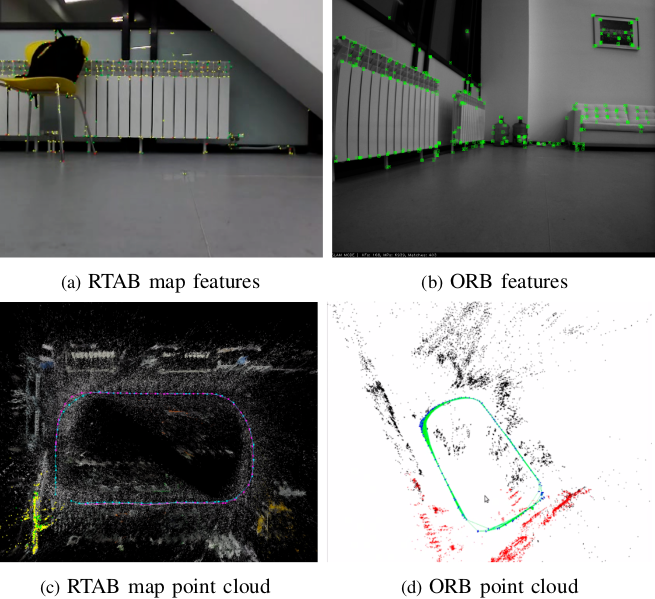
\includegraphics[width=0.5\textwidth]{comparaçãos.png}       
    \end{columns}
 %*----------- notes
    %\note[item]{Notes can help you to remember important information. Turn on the notes option.}
\end{frame}
%-
%*----------- SLIDE -------------------------------------------------------------
\begin{frame}[t]{Comparação}
    \transboxout[duration=0.5]
    %\framesubtitle{Darwin-OP}
    \begin{columns}
        \column{1\textwidth}
            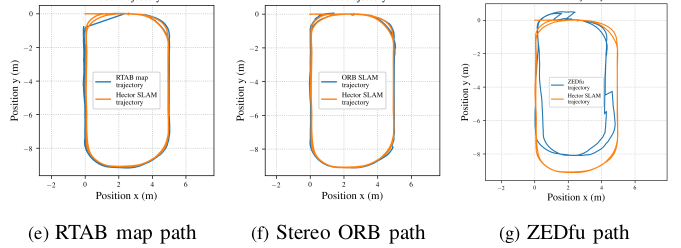
\includegraphics[width=1\textwidth]{comps.png}       
    \end{columns}
 %*----------- notes
    %\note[item]{Notes can help you to remember important information. Turn on the notes option.}
\end{frame}
%-
%*----------- SLIDE -------------------------------------------------------------
\begin{frame}[t]{Comparação}
    \transboxout[duration=0.5]
    %\framesubtitle{Darwin-OP}
    \begin{columns}
        \column{1\textwidth}
            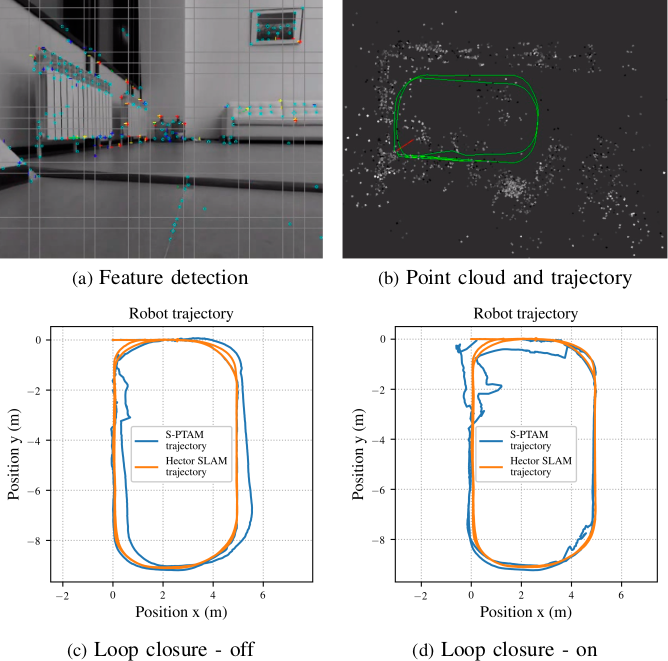
\includegraphics[width=0.5\textwidth]{comppss.png}       
    \end{columns}
 %*----------- notes
    %\note[item]{Notes can help you to remember important information. Turn on the notes option.}
\end{frame}
%-
%*----------- SLIDE -------------------------------------------------------------
\begin{frame}[t]{Comparação De Resultados}
    %\transboxin[duration=1,direction=30]
    \transboxout[duration=0.5]
    %\framesubtitle{Darwin-OP}
    \begin{columns}
        %\column{.1\textwidth}
        \column{.9\textwidth}
            \begin{enumerate}
                \item ZEDfu - Para a experiência forneceu RMSE grande, o sistema é robusto em termo de rastreamento de pose mas a trajetória não é exata para tal tipo de navegação.
                \item RTAB - Tem problema com a pose quando o robô se aproxima das paredes, mas o sistema de detecção de falha é capaz de detectar a falha e determinar a pose correta do robô. É robusto e preciso, tem precisão comparável com os métodos do lidar.
                \item ORB - Estimativa boa e cria mapas 3D esparso, localização robusta.
                \item PTAM - É robusto em termos de rastreio de pose e tem o mapa esparso, mas a precisão não é suficiente. 
            \end{enumerate}
    \end{columns}
%*----------- notes
    %\note[item]{Notes can help you to remember important information. Turn on the notes option.}
\end{frame}
%-
%*----------- SLIDE -------------------------------------------------------------
\begin{frame}[t]{Camera stéreo}
    \transboxout[duration=0.5]
    %\framesubtitle{Darwin-OP}
    \begin{columns}
        \column{1\textwidth}
            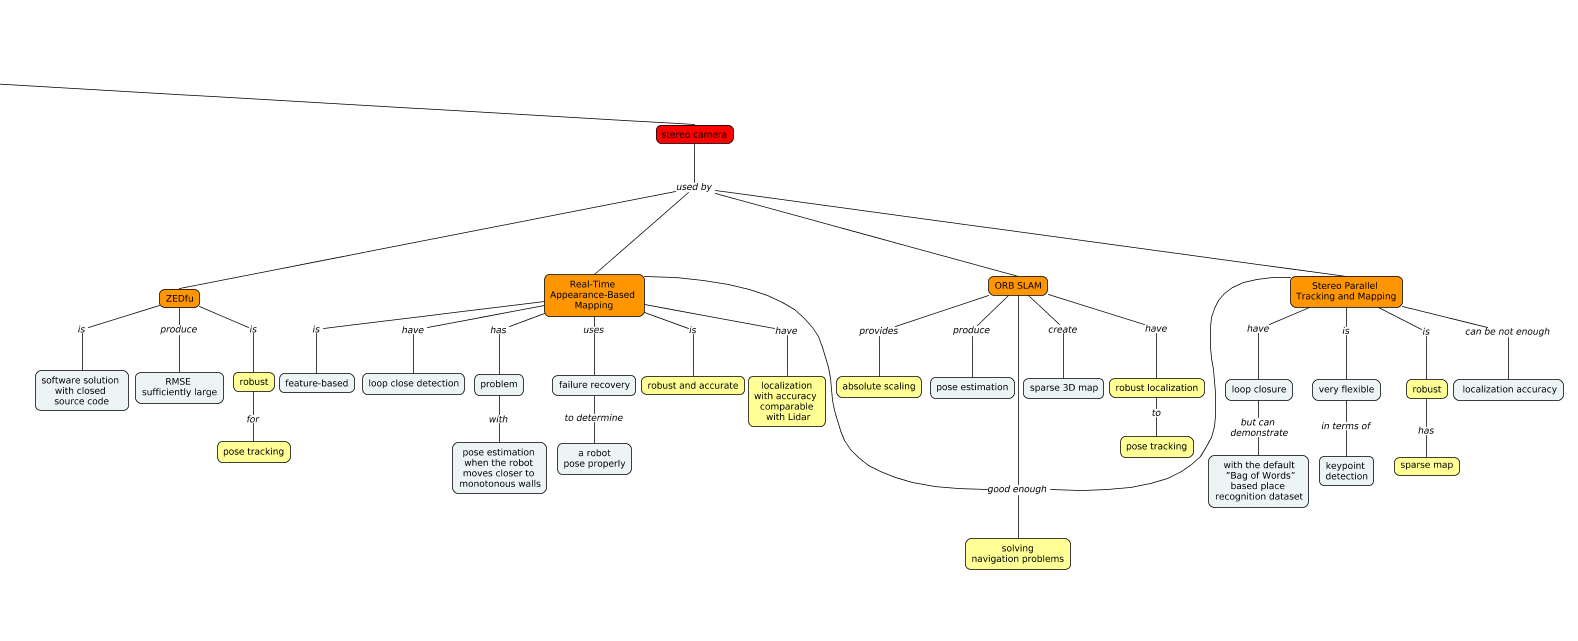
\includegraphics[width=1\textwidth]{mapa1.png}
    \end{columns}
 %*----------- notes
    %\note[item]{Notes can help you to remember important information. Turn on the notes option.}
\end{frame}
%-
%*----------- SLIDE -------------------------------------------------------------
\begin{frame}[t]{Camera stéreo}
    \transboxout[duration=0.5]
    %\framesubtitle{Darwin-OP}
    \begin{columns}
        \column{1\textwidth}
            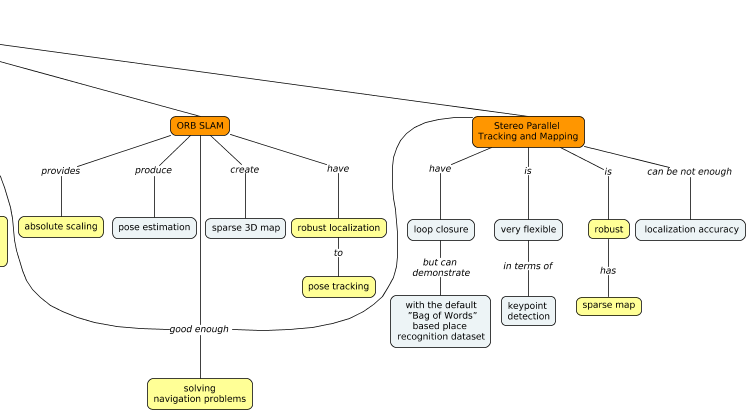
\includegraphics[width=.85\textwidth]{mapa4.png}
    \end{columns}
 %*----------- notes
    %\note[item]{Notes can help you to remember important information. Turn on the notes option.}
\end{frame}
%-
%*----------- SLIDE -------------------------------------------------------------
\begin{frame}[t]{Camera stéreo}
    \transboxout[duration=0.5]
    %\framesubtitle{Darwin-OP}
    \begin{columns}
        \column{1\textwidth}
            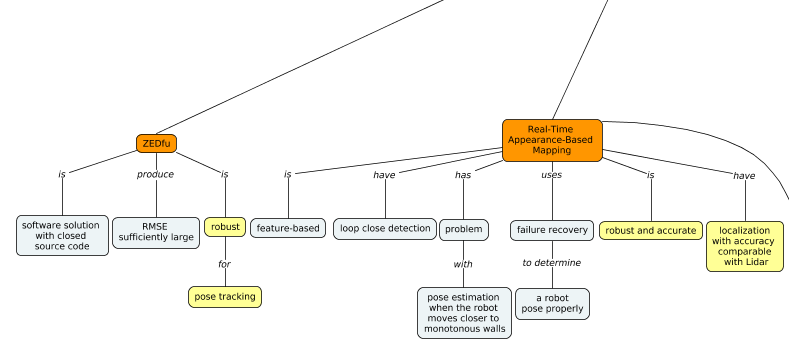
\includegraphics[width=1\textwidth]{mapa3.png}
    \end{columns}
 %*----------- notes
    %\note[item]{Notes can help you to remember important information. Turn on the notes option.}
\end{frame}
%-
%*----------- SLIDE -------------------------------------------------------------
\begin{frame}[t]{Comparação}
    \transboxout[duration=0.5]
    %\framesubtitle{Darwin-OP}
    \begin{columns}
        \column{1\textwidth}
            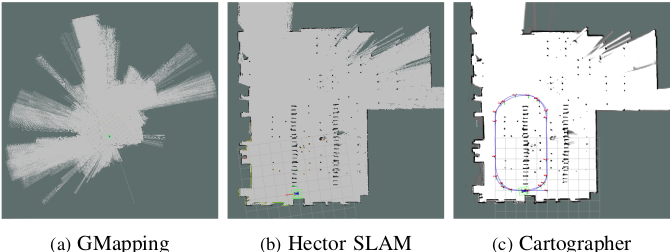
\includegraphics[width=.5\textwidth]{1.png}
            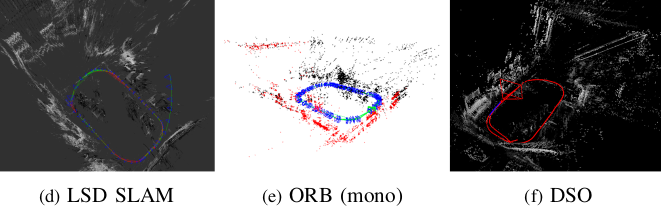
\includegraphics[width=.5\textwidth]{2.png}
            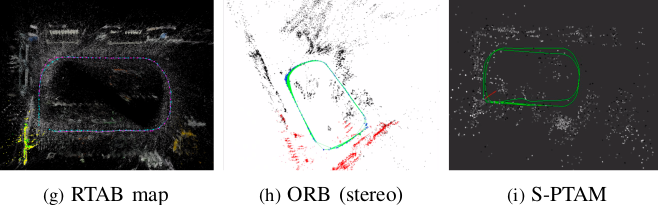
\includegraphics[width=.5\textwidth]{3.png}
    \end{columns}
 %*----------- notes
    %\note[item]{Notes can help you to remember important information. Turn on the notes option.}
\end{frame}
%-
%*----------- SLIDE -------------------------------------------------------------
\begin{frame}[t]{RESULTADO FILNAL}
    \transboxout[duration=0.5]
    %\framesubtitle{Darwin-OP}
    \begin{columns}
        \column{1\textwidth}
            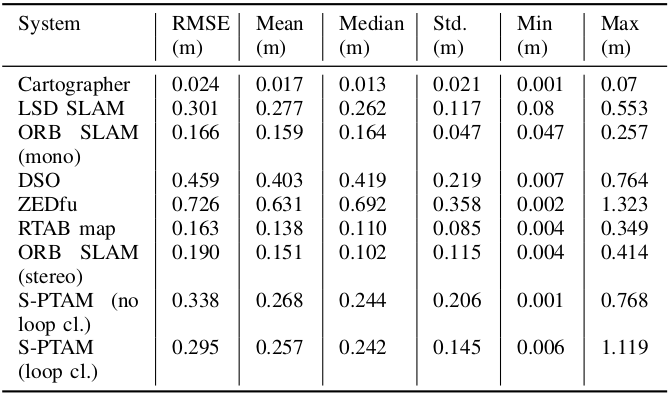
\includegraphics[width=0.7\textwidth]{result.png}
    \end{columns}
 %*----------- notes
    %\note[item]{Notes can help you to remember important information. Turn on the notes option.}
\end{frame}
%-
%*----------- SLIDE -------------------------------------------------------------
\begin{frame}[t]{RESULTADO FILNAL}
    \transboxout[duration=0.5]
    %\framesubtitle{Darwin-OP}
    \begin{columns}
        \column{1\textwidth}
            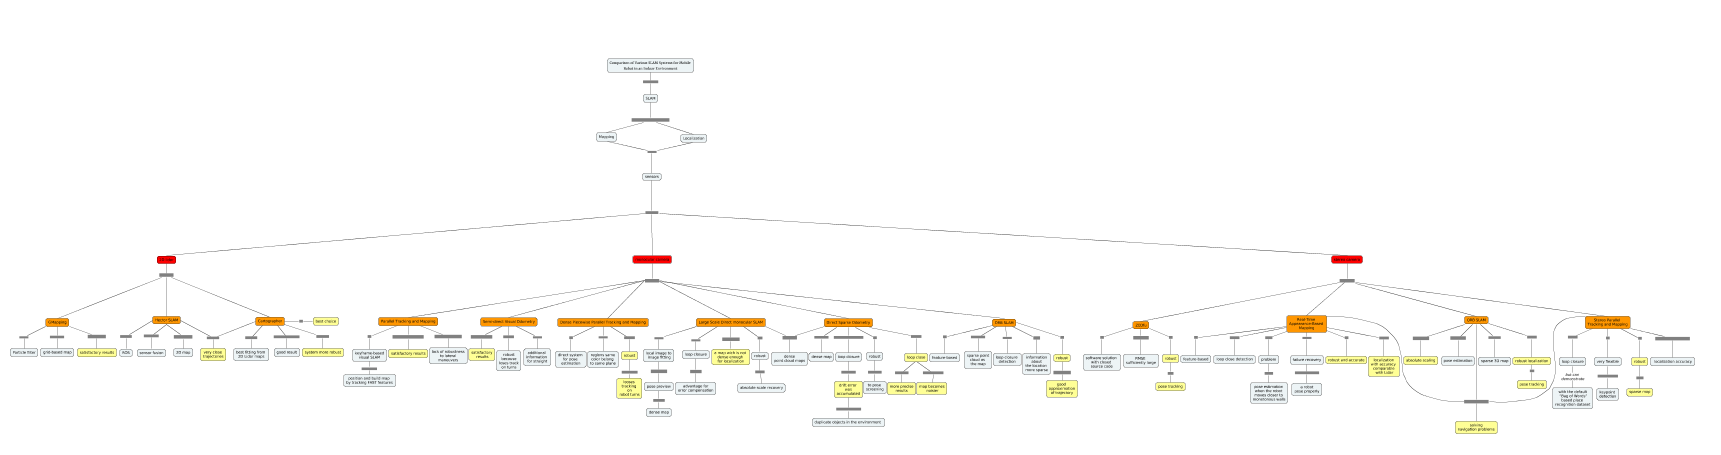
\includegraphics[width=1\textwidth]{ultimo.png}
    \end{columns}
 %*----------- notes
    %\note[item]{Notes can help you to remember important information. Turn on the notes option.}
\end{frame}
%-